% Chapter 4

\chapter{Design} % Main chapter title
\label{chap:Chapter4}

In this chapter is possible to find the progression of the solution design and the reasoning behind it.

\section{Use cases}

\dots %TODO

\section{Architecture}

To ensure quality, any solution needs a carefully planned architecture that accomplishes efficiently and effectively the already established requirements.
With this in mind, a component diagram was created to demonstrate all the components, and their interactions, that will compose the system.

\begin{figure}[H]
\centering
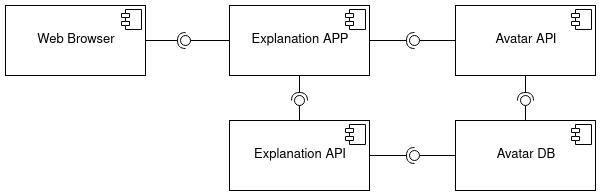
\includegraphics[scale=0.5]{ch4/assets/component_diagram.png}
\caption[Component Diagram]{Component Diagram}
\label{fig:cd}
\end{figure}

The architecture proposed to be implemented is shown in Figure~\ref{fig:cd}, it is composed by the following components:

\begin{itemize}
    \item Website - This component is responsible for the interactions of the users with the application.
    \item Explanation App - This component is responsible for processing the users input and converting the APIs output to the website.
    \item Explanation API - This component is responsible for generating an explanation for a given string.
    \item Avatar API - This component is responsible for converting a given string to \gls{LGP}.
    \item Avatar DB - This component is responsible for storing all the translations from Portuguese to \gls{LGP}.
\end{itemize}

\section{System Functionalities}

The first step to design a possible solution was to create a high-level view of the main functionalities the application should have.
% Vista de processo TODO
\begin{figure}[H]
\centering
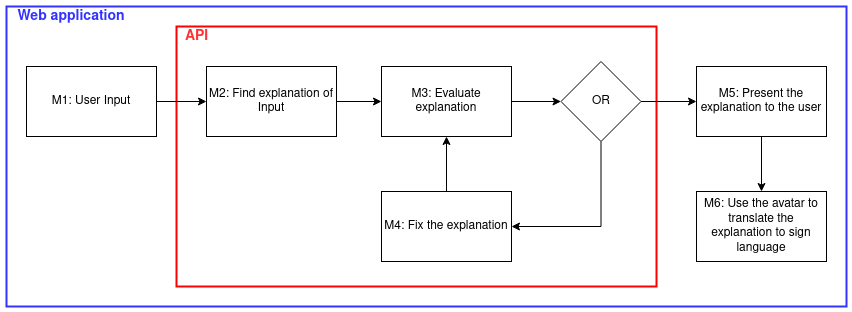
\includegraphics[scale=0.5]{ch4/assets/diagram1_2.png}
\caption[High-Level Approach]{High-Level Approach}
\label{fig:Diagram1}
\end{figure}

In the Figure~\ref{fig:Diagram1} is shown the main build blocks of the web application to be developed.
The input received in M1 is send to the \gls{API} that generates an explanation in M2, which is validated in M3.
From there the explanation might be sent back to the application and shown to the user in M5  or if does not meet all the criteria defined in M3 it will be fixed in M4 and reevaluated.
After presenting the explanation to the user, the application will also be capable of send the text to an already existing \gls{API} that is capable of translate plain text to \gls{LGP} using a avatar in M6.

To help better understand the created design, a more detailed view, is presented below, that describes each of the build blocks and how will they achieve the tasks previously mentioned.

\begin{figure}[H]
\centering
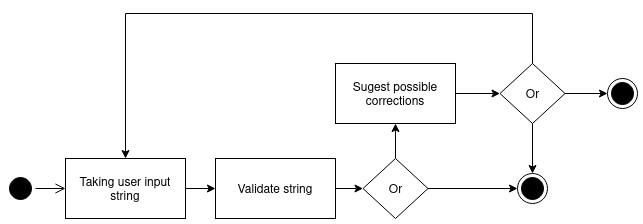
\includegraphics[scale=0.5]{ch4/assets/M1.png}
\caption[User Input Module]{M1: User Input}
\label{fig:M1}
\end{figure}

As shown in the Figure~\ref{fig:M1} the M1 block was design to receive a input string from the user.
This string is validated in order to detect common mistakes, such as typos, and when an mistake is detected the application suggests possible corrections.
The user is then capable of accepting the suggestion given, make a manual correction or proceed without changing the input string.

\begin{figure}[H]
\centering
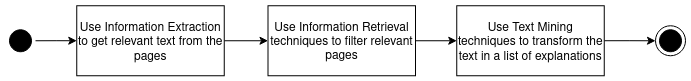
\includegraphics[scale=0.5]{ch4/assets/M2.png}
\caption[Find Explanation Module]{M2: Find Explanation}
\label{fig:M2}
\end{figure}

The Figure~\ref{fig:M2} the M2 block shows the process of finding an explanation based on the received string.
A web crawler would be use to find all the pages connected to a predefined starting page, such as Wikipedia or a dictionary.
From this point, Information Retrieval techniques would be used to filter the pages that may contain information that is related to the received string.
The filtered pages would then be processed using Information Extraction techniques in order to filter the text that has some degree of relation with the initial string.
An explanation will the be generated by implementing Text Mining techniques to the blocks of text obtained from the previous step.

\begin{figure}[H]
\centering
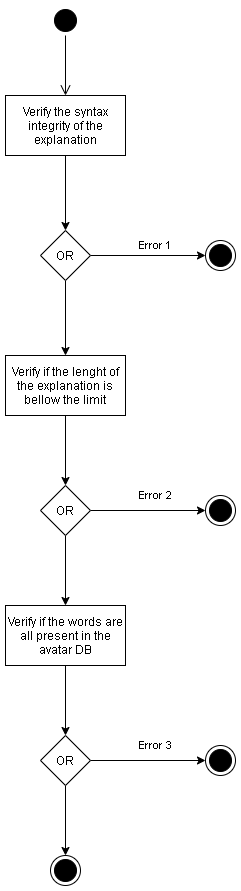
\includegraphics[scale=0.5]{ch4/assets/M3.png}
\caption[Evaluate Explanation Module]{M3: Evaluate Explanation}
\label{fig:M3}
\end{figure}

In Figure~\ref{fig:M3} the M3 block presents the evaluation criteria defined in order to defined an explanation as valid in order to be presented to the user.
Those criteria are the following:

\begin{itemize}
    \item Syntax integrity - The explanation follows syntax rules, or in other word, is a coherent sentence that can be understand when read.
    \item Word count limit - The explanation string needs to be shorter that a predefined value.
    \item Compatibility with the avatar \gls{DB} - The explanation string, ideally, needs to be composed only by words already exiting in the avatar \gls{DB}.
\end{itemize}

If a criterion fails, the error is set, and the process progresses with M4.
If a received explanation meets all the criteria it will be sent back to the web application, and the process progresses with M5.

\begin{figure}[H]
\centering
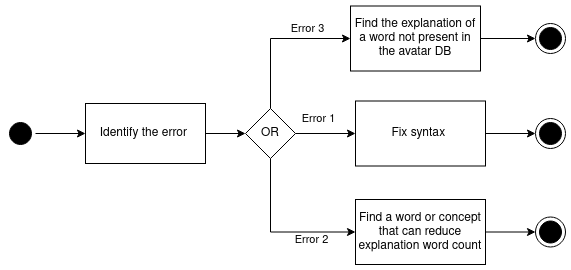
\includegraphics[width=\textwidth,keepaspectratio]{ch4/assets/M4.png}
\caption[Fix Explanation Module]{M4: Fix Explanation}
\label{fig:M4}
\end{figure}

As it can be seen in Figure~\ref{fig:M4} the M4 block is responsible for restructuring the explanation in order to meet the previously mention criteria.
It starts by identifying the error that made the explanation not be valid to progress and take action accordingly.

\begin{itemize}
    \item In order to fix a faulty syntax integrity, the string needs to be processed and restructured following syntax rules.
    \item In order to fix a string above a word count limit, the string need to be analyzed to, ideally, find a word or concept that can replace a portion of the string.
    \item In order to fix incompatibilities with the avatar \gls{DB}, the words that need to be replaced, a explanation might be generated and be presented as an hypermedia link to the missing word.
\end{itemize}

The new string will then be reevaluated by the M3 block.

\begin{figure}[H]
\centering
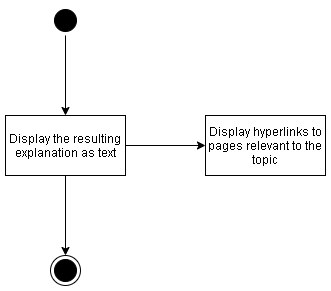
\includegraphics[scale=0.5]{ch4/assets/M5.png}
\caption[Present Explanation Module]{M5: Present Explanation}
\label{fig:M5}
\end{figure}

In the Figure~\ref{fig:M5} the M5 block will be displaying the generated explanation as text and hyperlinks to pages, related with the input string, to the user.
If the explanation had incompatibility issues in M3, then those faulty words will be also be presented as hypermedia with an explanation of them.

\begin{figure}[H]
\centering
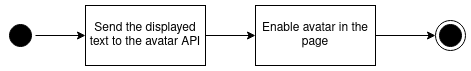
\includegraphics[scale=0.5]{ch4/assets/M6.png}
\caption[Avatar Module]{M6: Avatar}
\label{fig:M6}
\end{figure}

Shown in Figure~\ref{fig:M6} is the M6 block that will take the explanation text and send it to the avatar \gls{API}.
The avatar will appear in the web page, and will translate the received text to \gls{LGP}.

With the complete design of the application in mind a simpler and easier to implement approach was design, also known as a \gls{MVP}.

\begin{figure}[H]
\centering
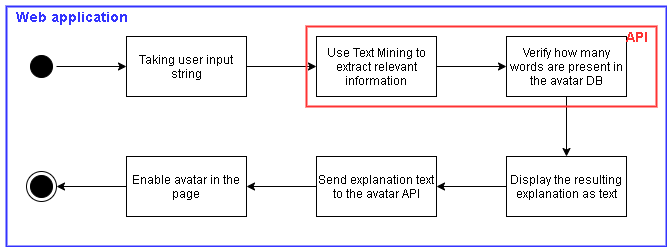
\includegraphics[scale=0.5]{ch4/assets/mvp_2.png}
\caption[Minimun Value Product]{Minimum Value Product}
\label{fig:mvp}
\end{figure}

The Figure~\ref{fig:mvp} shows the starting point of the solution to be developed.
As a \gls{MVP}, this design focus on the key functionalities that the solution must have, removing everything else.
The major benefit of choosing this approach is allowing a fast developed of a prototype that can be used to receive feedback from the target audience, in order to grantee that the solution is going towards their needs.

\section{Design alternatives}

The main goal was initial the development of a web application that was capable of showing the users an explanation of a word or expression.
Like so the application was envisioned to take the input generate the explanation and show it to the user, like its shown in Figure~\ref{fig:ocd}.

\begin{figure}[H]
\centering
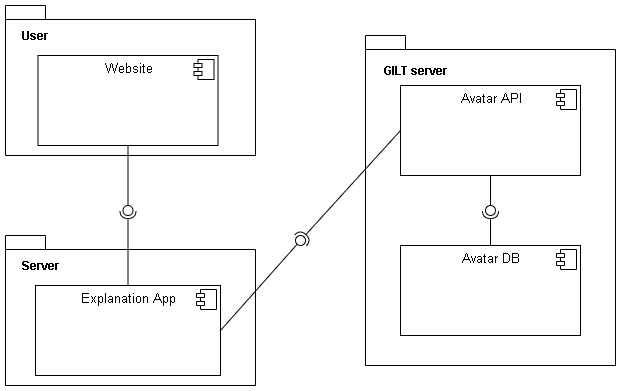
\includegraphics[scale=0.5]{ch4/assets/component_diagram_old.png}
\caption[Old Component Diagram]{Old Component Diagram}
\label{fig:ocd}
\end{figure}

The disadvantage of this design in comparison with the one previously presented is that, in this one, the back end of the web application would produce the explanation.
This wouldn't allow to easily reutilize the main functionality of the application which is the generation of an explanation.
In GILT there are projects that would benefit from this feature and therefore the design had to be changed.
